\documentclass{article}

\usepackage{graphicx}
\usepackage{hyperref}
\usepackage{listings}
\usepackage{color}
\usepackage{verbatim}
%\usepackage{subfigure}
\usepackage{amsmath}
\usepackage{caption}
\usepackage{subcaption}



\begin{document}
\title{Eric Buras Thesis: Results}

\maketitle

\section{Graphs}
We have a set of graphs that are similar to the power-law graphs from Watts-Strogatz and Chung-Lu. These encompass a wide range of subjects such as social networks, biological processes, and an electric grid. The key part of my algorithm is partitioning a graph into a large locally-connected subgraph and a small teleportation subgraph. four of these examples fully fit into this class of graphs, whereas the power grid most certainly does not as evidenced below. The important attribute to look for is low rank of the teleportation Laplacian matrix relative to the number of the nodes (which is the size of the entire square Laplacian matrix).\\


\begin{figure}
\centering

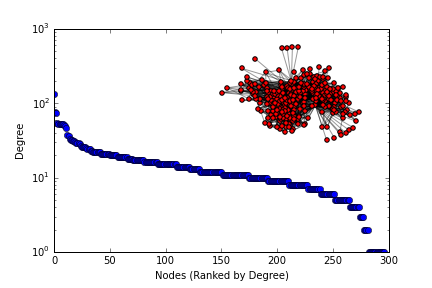
\includegraphics[width=\linewidth]{neural_degree_histogram.png}
\caption{Neural Network of C. Elegans \cite{White:1986,Watts:1998}}
  
\end{figure}

\begin{figure}
\centering
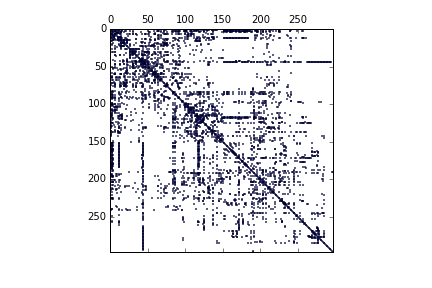
\includegraphics[width = \linewidth]{neuralspy.png}
\caption{Spy Plot of Neural Network Laplacian Matrix}
\end{figure}

\begin{figure}
\centering

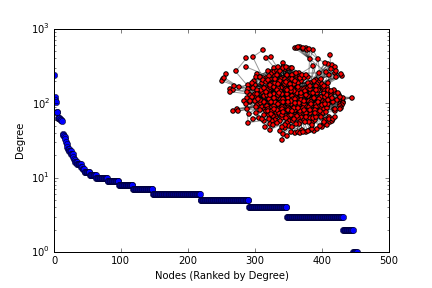
\includegraphics[width=\linewidth]{meta_degree_histogram.png}
\caption{Metabolic Network of C. Elegans \cite{Duch:2005}}
  
\end{figure}
\begin{figure}
\centering
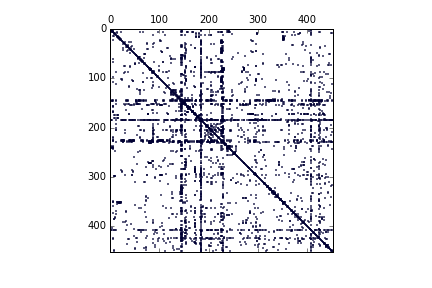
\includegraphics[width = \linewidth]{metaspy.png}
\caption{Spy Plot of Metabolic Network Laplacian Matrix}
\end{figure}

\begin{figure}
\centering

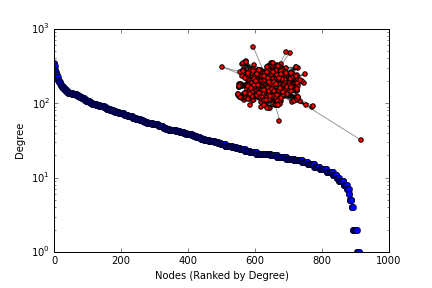
\includegraphics[width=\linewidth]{gene_degree_histogram.png}
\caption{Gene Network Encoding Proteins of C. Elegans \cite{Simonis:2009}}
  
\end{figure}

\begin{figure}
\centering
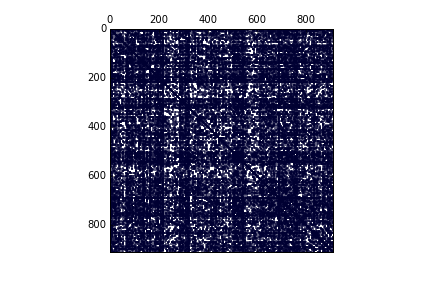
\includegraphics[width = \linewidth]{genespy.png}
\caption{Spy Plot of Gene Network Laplacian Matrix}
\end{figure}

\begin{figure}
\centering

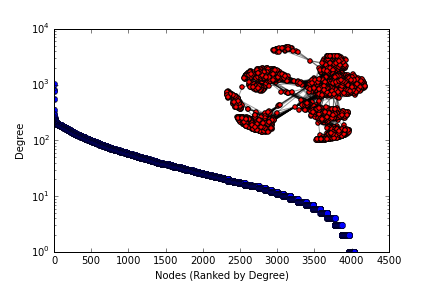
\includegraphics[width=\linewidth]{fb_degree_histogram.png}
\caption{Facebook Friend Network \cite{Mcauley:2012}}
  
\end{figure}

\begin{figure}
\centering
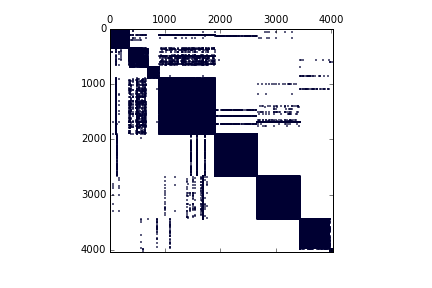
\includegraphics[width = \linewidth]{fbspy.png}
\caption{Spy Plot of Facebook Network Laplacian Matrix}
\end{figure}

\begin{figure}
\centering

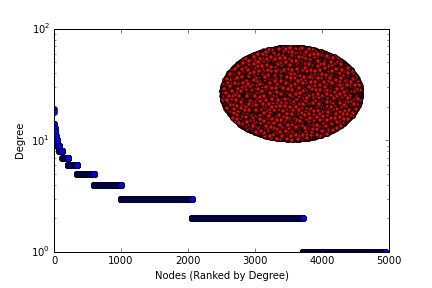
\includegraphics[width=\linewidth]{power_degree_histogram.png}
\caption{Network of Western Power Grid \cite{Watts:1998}}
  
\end{figure}

\begin{figure}
\centering
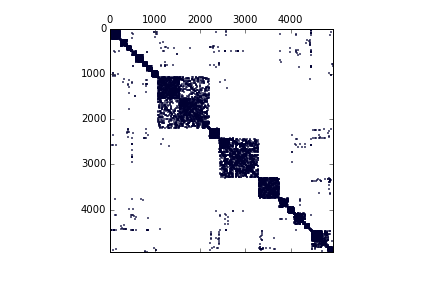
\includegraphics[width = \linewidth]{powerspy.png}
\caption{Spy Plot of Power Grid Laplacian Matrix}
\end{figure}


\begin{center}
\renewcommand{\arraystretch}{1.5}
    \begin{tabular}{| l | l | l | l | l | l |}
    \hline
    Graph (nodes, edges) & Avg. Deg. & Rank $T_L$ & Nx part. (s) & Part. (s) & Iter. \\ \hline
    Neural (297, 2148) & 14.46 & 22 & 11 & 1.6 & 2 \\ \hline
    Metabolic (453, 2025) & 8.94 & 49 & 12 & 2.3 & 2 \\  \hline
    Gene (912, 22738) & 49.86 & 26 & 1915 & 53 & 1 \\ \hline
    Facebook (4039, 88234) & 43.69 &  180 & 11593 & 480 & 2 \\ \hline
    Power (4941, 6594) & 2.669 & 4284 & 2.1 & .33 & 2 \\ 
    \hline
    \end{tabular}
\end{center}
I want to dig deeper into the solve portion to determine if the operations correspond with their given theoretical complexities. Here is a table of the timings for the individual operations:\\

\begin{center}
\renewcommand{\arraystretch}{1.5}
    \begin{tabular}{ | l | l | l | l | l | l | l |}
    \hline
    \textbf{Operation} & \textbf{Order} & \textbf{Neural} & \textbf{Meta} & \textbf{Gene} & \textbf{FB} & \textbf{Power} \\ \hline
    $USV = T_L$ & $O(n^3)$ & .0334 & .0737 & .4183 & 38.47 & 72.86  \\ \hline
    $S^{-1}$ & $O(r)$ & .0005 & .0007 & .0001 & .0023 & 5.104 \\ \hline
    $y = P_L^{-1}b$ (MG) & $O(n)$ & .0857 & .0962 & .3552 & 1.347 & .1152  \\  \hline
    $y_1 = Vy$ & $O(rn)$ & .0013 & .0015 & .0002 & .0023 & .0702 \\ \hline
    $Q = P_L^{-1}U$ ($r\times$MG) & $O(rn)$ & .3292 & .7360 & .5190 & 23.11 & 106.9  \\ \hline
    $Q_1 = VQ$ & $O(r^2 n)$ & .0006 & .0036 & .0013 & .4124 & 285.1 \\ \hline
    $Q_2 = S^{-1} + Q_1$ & $O(r^2)$ & .0012 & .0018 & .0003 & .0011 & .4157 \\ \hline
    $y_2 = Q_2^{-1}y_1$ & $O(r^3)$ & .0023 & .0025 & .0013 & .0099 & 86.49 \\ \hline
    $y_3 = Uy_2$ & $O(rn)$ & .0001 & .0002 & .0003 & .0025 & .1867 \\ \hline
    $y_4 = P_L^{-1}y_3$ (MG) & $O(n)$ &.0128 & .0070 & .1183 & .8249 & .0059 \\ \hline
    $x = y - y_4$ & $O(n)$ &.0003 & .0003 & .0003 & .0004 & .0003 \\ \hline
    \textbf{Total} & $O(n^3)$ & .51 & .966 & 1.44 & 64.46 & 560 \\
    \hline
    \end{tabular}
\end{center}
As observed, the operation timings correspond to their theoretical floating point operation orders. For the first four examples (not including the power grid solve), the limiting operations are the singular value decomposition and multiple right hand side multigrid solves, $Q = P_L^{-1}U$. These operations can be optimized using the low-rank SVD and by vectorizing the multiple right hand solves so that only one multigrid solve must be done. However for the full rank power-grid solve, the limiting operations are the SVD, the matrix-matrix multiplication, $Q_1 = VQ$, and the matrix solve, $y_2 = Q_2^{-1}y_1$. Graph Laplacian linear systems without low-rank $T_L$ should not be solved using this method.

\bibliographystyle{plain}
\bibliography{mastersbib}
\end{document}